%%%%%%%%%%%%%%%%%%%%%%%%%%%%%%%%%%%%%%%%%
% Wenneker Assignment
% LaTeX Template
% Version 2.0 (12/1/2019)
%
% This template originates from:
% http://www.LaTeXTemplates.com
%
% Authors:
% Vel (vel@LaTeXTemplates.com)
% Frits Wenneker
%
% License:
% CC BY-NC-SA 3.0 (http://creativecommons.org/licenses/by-nc-sa/3.0/)
% 
%%%%%%%%%%%%%%%%%%%%%%%%%%%%%%%%%%%%%%%%%

%----------------------------------------------------------------------------------------
%	PACKAGES AND OTHER DOCUMENT CONFIGURATIONS
%----------------------------------------------------------------------------------------

\documentclass[11pt]{scrartcl} % Font size

%%%%%%%%%%%%%%%%%%%%%%%%%%%%%%%%%%%%%%%%%
% Wenneker Assignment
% Structure Specification File
% Version 2.0 (12/1/2019)
%
% This template originates from:
% http://www.LaTeXTemplates.com
%
% Authors:
% Vel (vel@LaTeXTemplates.com)
% Frits Wenneker
%
% License:
% CC BY-NC-SA 3.0 (http://creativecommons.org/licenses/by-nc-sa/3.0/)
% 
%%%%%%%%%%%%%%%%%%%%%%%%%%%%%%%%%%%%%%%%%

%----------------------------------------------------------------------------------------
%	PACKAGES AND OTHER DOCUMENT CONFIGURATIONS
%----------------------------------------------------------------------------------------

\usepackage{amsmath, amsfonts, amsthm} % Math packages

\usepackage{listings} % Code listings, with syntax highlighting
\usepackage[outputdir=out]{minted}

\usepackage[english]{babel} % English language hyphenation

\usepackage{graphicx} % Required for inserting images
\graphicspath{{Figures/}{./}} % Specifies where to look for included images (trailing slash required)

\usepackage{booktabs} % Required for better horizontal rules in tables

\numberwithin{equation}{section} % Number equations within sections (i.e. 1.1, 1.2, 2.1, 2.2 instead of 1, 2, 3, 4)
\numberwithin{figure}{section} % Number figures within sections (i.e. 1.1, 1.2, 2.1, 2.2 instead of 1, 2, 3, 4)
\numberwithin{table}{section} % Number tables within sections (i.e. 1.1, 1.2, 2.1, 2.2 instead of 1, 2, 3, 4)

\setlength\parindent{0pt} % Removes all indentation from paragraphs

\usepackage{enumitem} % Required for list customisation
\setlist{noitemsep} % No spacing between list items

%----------------------------------------------------------------------------------------
%	DOCUMENT MARGINS
%----------------------------------------------------------------------------------------

\usepackage{geometry} % Required for adjusting page dimensions and margins

\geometry{
	paper=a4paper, % Paper size, change to letterpaper for US letter size
	top=2.5cm, % Top margin
	bottom=3cm, % Bottom margin
	left=3cm, % Left margin
	right=3cm, % Right margin
	headheight=0.75cm, % Header height
	footskip=1.5cm, % Space from the bottom margin to the baseline of the footer
	headsep=0.75cm, % Space from the top margin to the baseline of the header
	%showframe, % Uncomment to show how the type block is set on the page
}

%----------------------------------------------------------------------------------------
%	FONTS
%----------------------------------------------------------------------------------------

\usepackage[utf8]{inputenc} % Required for inputting international characters
\usepackage[T1]{fontenc} % Use 8-bit encoding

\usepackage{fourier} % Use the Adobe Utopia font for the document

%----------------------------------------------------------------------------------------
%	SECTION TITLES
%----------------------------------------------------------------------------------------

\usepackage{sectsty} % Allows customising section commands

\sectionfont{\vspace{6pt}\centering\normalfont\scshape} % \section{} styling
\subsectionfont{\normalfont\bfseries} % \subsection{} styling
\subsubsectionfont{\normalfont\itshape} % \subsubsection{} styling
\paragraphfont{\normalfont\scshape} % \paragraph{} styling

%----------------------------------------------------------------------------------------
%	HEADERS AND FOOTERS
%----------------------------------------------------------------------------------------

\usepackage{scrlayer-scrpage} % Required for customising headers and footers

\ohead*{} % Right header
\ihead*{} % Left header
\chead*{} % Centre header

\ofoot*{} % Right footer
\ifoot*{} % Left footer
\cfoot*{\pagemark} % Centre footer
 % Include the file specifying the document structure and custom commands

%----------------------------------------------------------------------------------------
%	TITLE SECTION
%----------------------------------------------------------------------------------------

\title{	
	\normalfont\normalsize
	\begin{center}
		\begin{minipage}[c]{0.2\textwidth}
			\textsc{\Large SZ-Ybbs}
		\end{minipage}%
		\begin{minipage}[c]{0.1\textwidth}
			
\includegraphics[width=\textwidth]{LogoITHTL_white.pdf}
		\end{minipage}
	\end{center}
	\vspace{10pt} % Whitespace
	\rule{\linewidth}{0.5pt}\\ % Thin top horizontal rule
	\vspace{20pt} % Whitespace
	{\huge TLS}\\ % The assignment title
	\vspace{12pt} % Whitespace
	\rule{\linewidth}{2pt}\\ % Thick bottom horizontal rule
	\vspace{12pt} % Whitespace
}

\author{\LARGE Erber Jakob, Freunberger Raphael} % Your name

\date{\normalsize\today} % Today's date (\today) or a custom date

\begin{document}

\maketitle % Print the title

\section{TLS Overview}

Transport Layer Security (TLS) is a cryptographic protocol used for providing secure communications over an insecure network, like the internet. TLS provides security, confidentiality, authenticity and integrity. TSL builds on top of the now-deprecated Secure Sockets Layer (SSL) protocol and does not clearly fit one OSI-layer. Depending on who you ask TLS can be categorized as either one of the layers 4, 5, 6 and 7. 
% Layer 5 (session layer): https://de.wikipedia.org/wiki/Transport_Layer_Security#TLS-Protokolle_im_Protokollstapel
% Layer 6 (presentation layer): https://en.wikipedia.org/wiki/Transport_Layer_Security
TLS uses TCP, but there is also a UDP equivalent called Datagram Transport Layer Security (DTLS). DTLS is sometimes used for VPNs but in general used less than TLS. TLS has a wide range of use cases, from email to voice over IP or web browsing.
\\\\
To keep its promise of security TLS has to keep being developed and new versions get released as the older versions become insecure and get deprecated. This table shows when each version was released and its current status.

\begin{table}[h]
    \centering
    \begin{tabular}{|l|c|l|}
        \hline
        \textbf{Version} & \textbf{Year} & \textbf{Status} \\ \hline
        TLS 1.0 (insecure) & 1999 & Deprecated in 2021 (RFC 8996) \\ \hline
        TLS 1.1 (insecure) & 2006 & Deprecated in 2021 (RFC 8996) \\ \hline
        TLS 1.2 & 2008 & In use since 2008 \\ \hline
        TLS 1.3 & 2018 & In use since 2018 \\ \hline
    \end{tabular}
    \caption{TLS Versions and Status}
    \label{tab:tls_versions}
\end{table}

\subsection{TLS supported ciphers}
\label{sec:tls_supported_ciphers}

This table shows the supported ciphers for the different TLS versions. It also shows which ciphers are secure and which are not. The information is taken from wikipedia. This table will be used later to compare the security of the different TLS versions and supported ciphers.

\begin{table}[H]
    \centering
    \renewcommand{\arraystretch}{1.3}
    \begin{tabular}{|p{2cm}|p{3cm}|p{2cm}|p{2cm}|p{2cm}|p{2cm}|}
        \hline
        \textbf{Type} & \textbf{Algorithm} & \textbf{TLS 1.0} & \textbf{TLS 1.1} & \textbf{TLS 1.2} & \textbf{TLS 1.3} \\ \hline
        
        \multirow{6}{*}{Block} & AES GCM & — & — & Secure & Secure \\ \cline{2-6}
         & AES CCM & — & — & Secure & Secure \\ \cline{2-6}
         & AES CBC & Insecure & Depends on mitigations & Depends on mitigations & — \\ \cline{2-6}
         & Camellia GCM & — & — & Secure & — \\ \cline{2-6}
         & Camellia CBC & Insecure & Depends on mitigations & Depends on mitigations & — \\ \cline{2-6}
         & ARIA GCM & — & — & Secure & — \\ \cline{2-6}
         & ARIA CBC & — & Depends on mitigations & Depends on mitigations & — \\ \cline{2-6}
         & SEED CBC & Insecure & Depends on mitigations & Depends on mitigations & — \\ \cline{2-6}
         & 3DES EDE CBC & Insecure & Insecure & Insecure & — \\ \cline{2-6}
         & GOST R 34.12-2015 Magma CTR & — & — & Insecure & — \\ \cline{2-6}
         & GOST R 34.12-2015 Kuznyechik CTR & — & — & Secure & — \\ \cline{2-6}
         & GOST R 34.12-2015 Magma MGM & — & — & — & Insecure \\ \cline{2-6}
         & GOST R 34.12-2015 Kuznyechik MGM & — & — & — & Secure \\ \cline{2-6}
         & IDEA CBC & Insecure & Insecure & Insecure & — \\ \cline{2-6}
         & DES CBC (56) & Insecure & Insecure & Insecure & — \\ \cline{2-6}
         & DES CBC (40) & Insecure & Insecure & — & — \\ \cline{2-6}
         & RC2 CBC & Insecure & Insecure & — & — \\ \hline
         
        \multirow{2}{*}{Stream} & ChaCha20-Poly1305 & — & — & Secure & Secure \\ \cline{2-6}
         & RC4 (128) & Insecure & Insecure & Insecure & — \\ \cline{2-6}
         & RC4 (40) & Insecure & Insecure & — & — \\ \hline
         
        None & Null & Insecure & Insecure & Insecure & — \\ \hline
    \end{tabular}
    \caption{Protocol Version Compatibility of Various Ciphers}
\end{table}


\section{Protocols}
\subsection{TLS 1.0 and 1.1}
TLS 1.0 was only a minor change from SSL 3.0, according to Tim Eireks, the minor changes and the renaming from ``SSL'' to ``TLS'' were a face-saving gesture to Microsoft, ``so it wouldn't look [like] the IETF was just rubberstamping Netscape's protocol''. The protocol is defined in RFC 2246.
\\
TLS 1.1 was only a minor change. The changes concerning security were the replacement of the implicit initial vector (IV) with an explicit IV, to protect against cipher block chaining attacks, and changing the handling of padding errors. The protocol is defined in RFC 4346.
\\\\
Both TLS 1.0 and 1.1 were deprecated in 2021, in RFC 8996, because both versions used SHA-1 for security purposes, and lack support for modern ciphers.

\subsection{TLS 1.2}

TLS 1.2 was released in 2008 and is still considered to be secure, depending on the cipher used. Its biggest change compared to TLS 1.1 is the replacement of the MD5 and SHA-1 hash functions with SHA-256 for all security uses and the support for more modern ciphers like AES GCM. However TLS 1.2 can still use a MD5 or SHA-1 HMAC for data integrity. TLS 1.2 is still widely used and supported by most modern web browsers and servers. The protocol is defined in RFC 5246.
\\\\
In 2011 refinements defined in RFC 6176 removed the backward compatibility with SSL 2.0.

\subsection{TLS 1.3}

TLS 1.3 was the largest change in the history of TLS. The TLS 1.3 requirement for forward secrecy meant that a lot of the previously supported key exchange/agreement algorithms were no longer supported. The only key exchange/agreement algorithms supported by TLS 1.3 are different versions of Diffie-Hellman (DH), Elliptic Curve Diffie-Hellman (ECDH) and one algorithm from the Russian GOST standards organization. The protocol is defined in RFC 8446.
\\\\
With previous TLS versions the encryption and data integrity algorithms were separate. The MAC was computed and appended to the data, then data+MAC were encrypted. However, this has security downsides. TLS 1.3 combined the encryption and data integrity algorithms, only supporting ciphers that use AEAD for data integrity. The supported cipher can be seen in \ref{sec:tls_supported_ciphers}.
\\\\
One of the other major changes, the new handshake protocol, will be discussed separately in \ref{sec:tls_handshake}.
\\\\
Where as the security of TLS 1.2 depends on the used cipher and key exchange method, TLS 1.3 only supports currently secure methods (expect one of the Russian GOST ciphers).
\\\\
Forward secrecy, sometimes also called perfect forward secrecy is a major change with TLS 1.3. Forward secrecy means that if the long term secrets used for the session, like the private key, are compromised, and the attacker recorded the entire encrypted session, they still can't decrypt the session.
\\
Forward secrecy is achieved by using a version of the Diffie Hellman key exchange instead of the client generating a secret key and sending it to the server encrypted with the server's public key. Because the server and client never send the secret key over the network, and the server's private key is no longer a factor in the key generation, an attacker can't decrypt the session if they get the long term secrets.

\section{Subprotocols}

\subsection{Handshake Protocol}

\subsection{Alert Protocol}

\subsection{ChangeCipherSpec Protocol}

\subsection{Application Protocol}



\section{TLS 1.2/1.3 Handshake}
\label{sec:tls_handshake}
First, we will go over the handshake that TLS 1.2 and prior versions used. In this example the server uses a certificate to prove its identity to the client, but the client does not use a certificate.
\\\\
This illustration shows the entire handshake process, including the TCP handshake, which is not directly part of the TLS handshake, but still contributes to TLS latency. 

\begin{figure}[H]
    \centering
    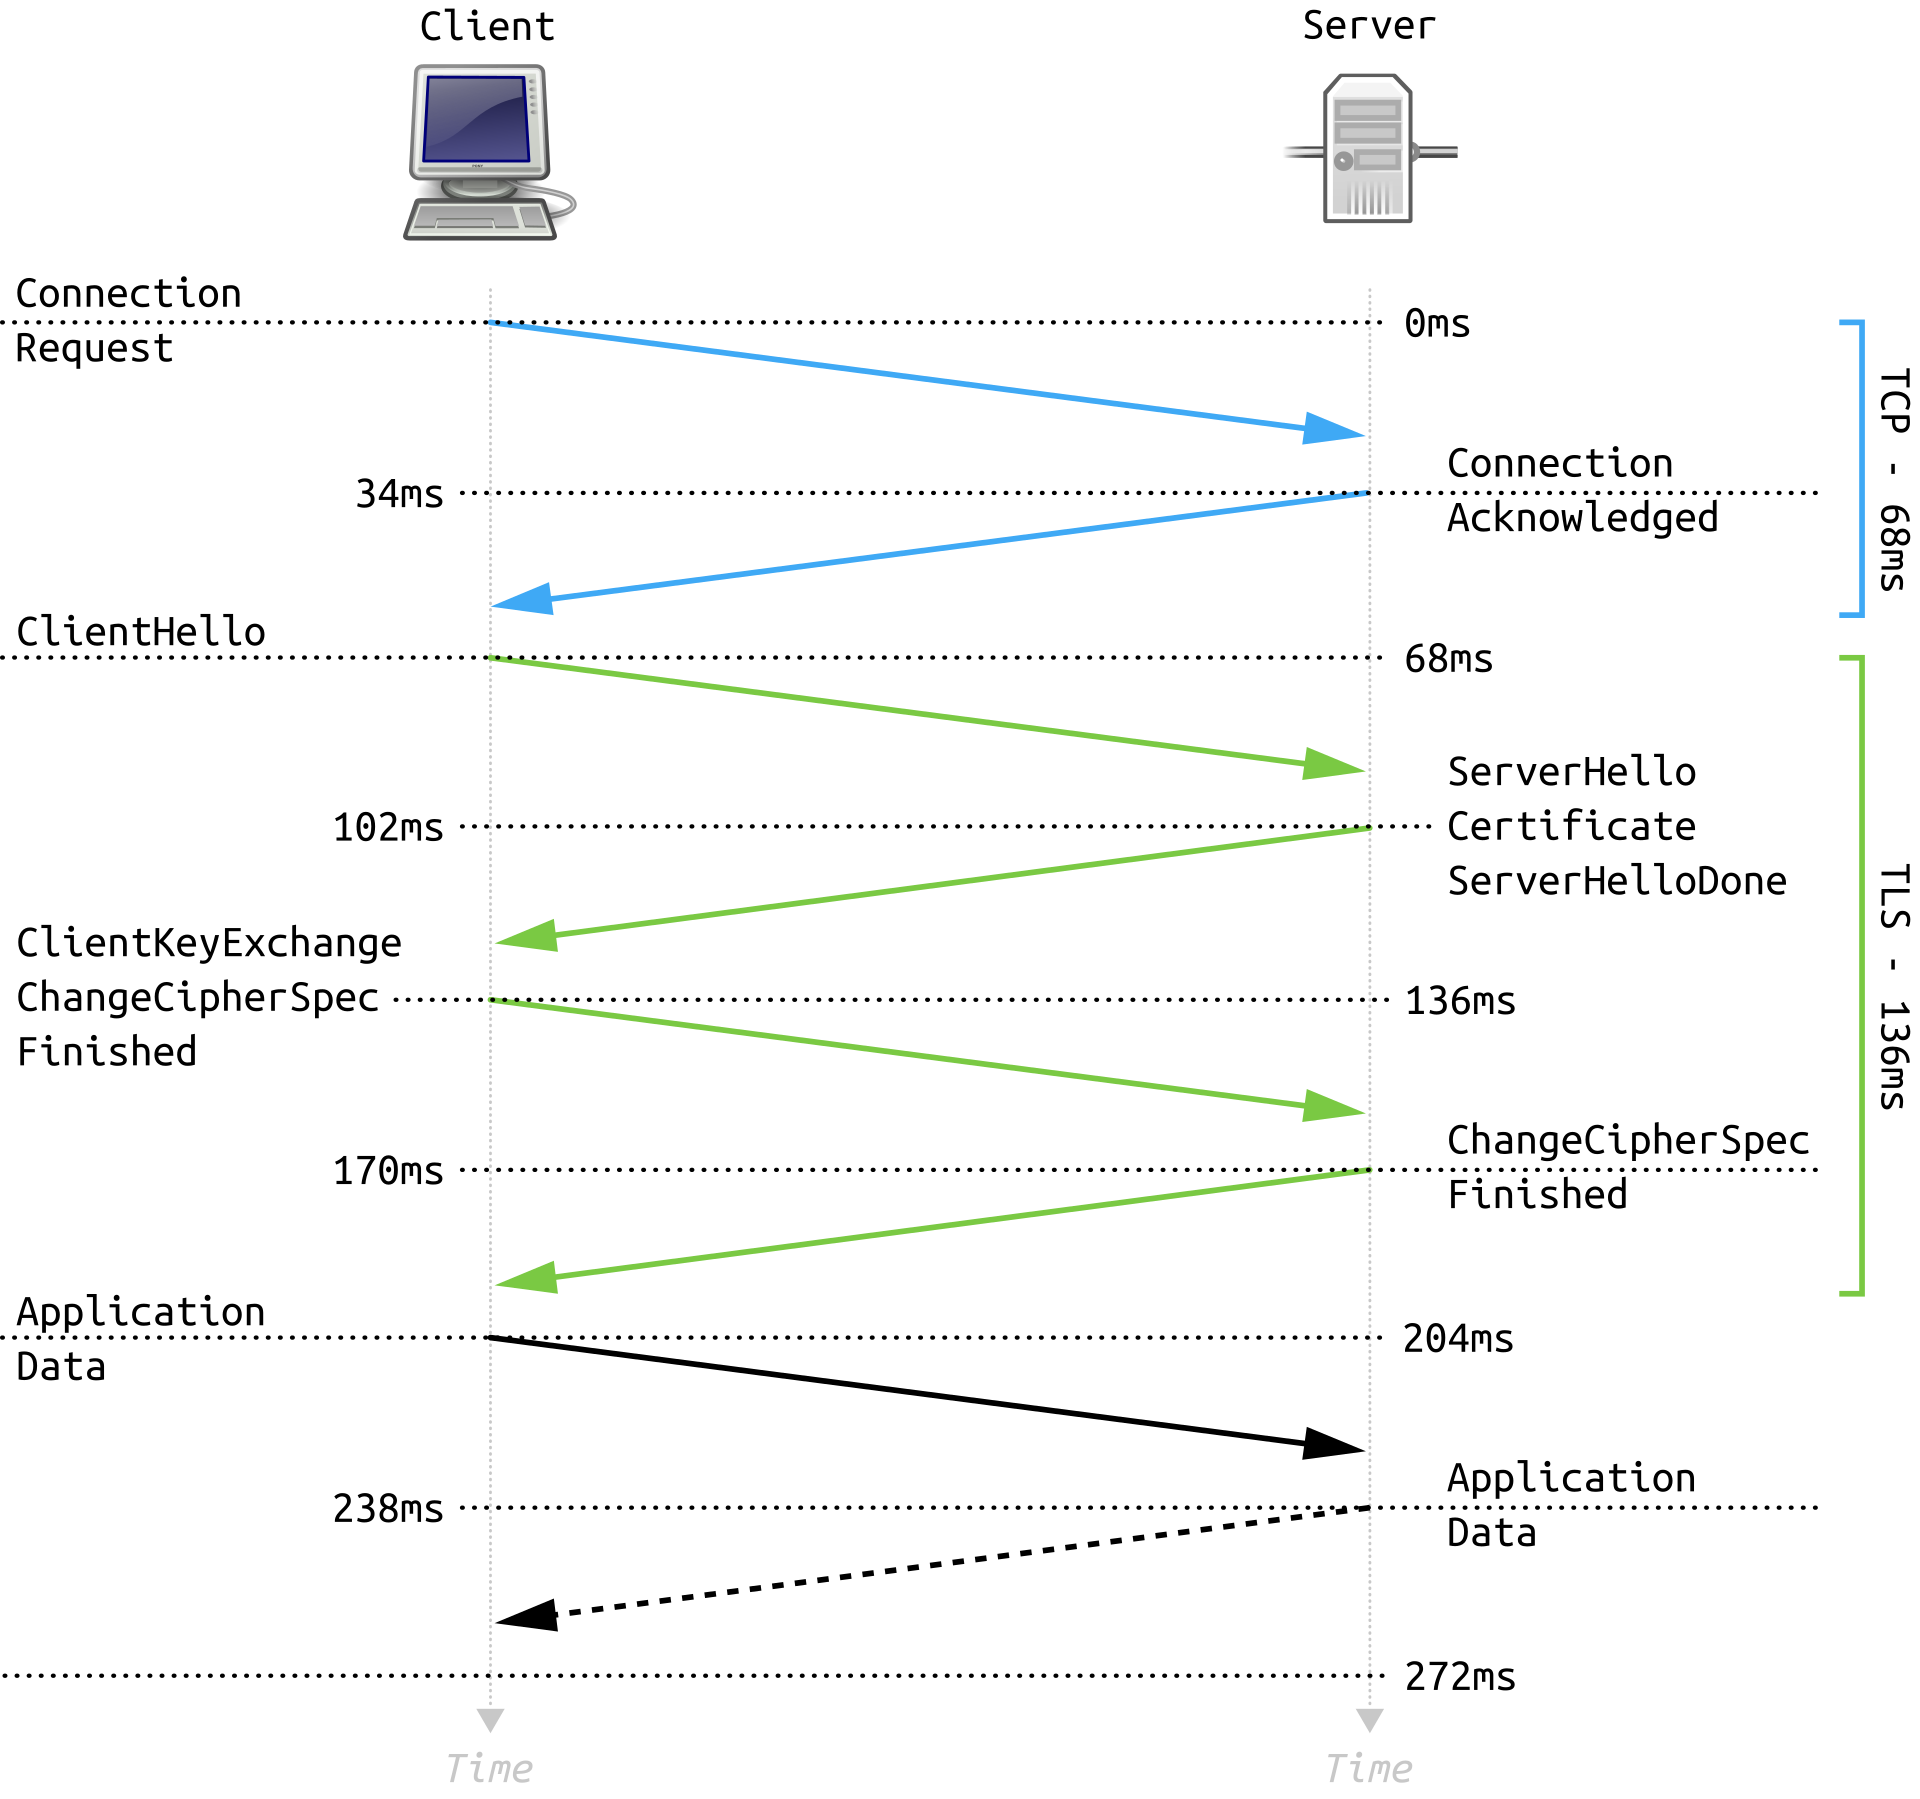
\includegraphics[width=0.8\textwidth]{Figures/Full_TLS_1_2_Handshake.png}
    \caption{TLS 1.2 Handshake}
    \label{fig:tls_handshake}
\end{figure}

The handshake can be separated into four phases:
\begin{enumerate}
    \item Negotiation: The client starts the handshake by sending a \texttt{ClientHello} message. The message contains the client's supported TLS versions, a list of supported ciphers, a random number and suggested compression methods.
    \\\\
    The server responds with a \texttt{ServerHello} message. The message contains the chosen TLS version, a chosen cipher, a random number and a chosen compression method from the supported ones the client sent before.
    \\
    The server also sends its certificate, which contains the server's public key.
    \\
    If the cipher is a version of Diffie Hellman, the server will also send a \texttt{ServerKeyExchange} message.
    \\
    The server also sends a \texttt{ServerHelloDone} message, which signals that the server is done with the negotiation phase.
    \\\\
    The client then sends a \texttt{ClientKeyExchange} message, which, depending on cipher used, contains the pre-master secret encrypted by the public key of the server, public key, or nothing.
    \\\\
    The server and client then compute a common secret, using the random numbers they shared and the pre-master secret. The common secret is also called master secret and is used to derive all other keys, like the session key or MAC key.
    
    \item The Clients sends a \texttt{ChangeCipherSpec} message, which signals that the client will start using the negotiated cipher and compression method.
    \\
    The client sends a encrypted \texttt{Finished} message, which contains a hash of all previous messages. The server will then try to decrypt the message and check if the hash is correct. If the hash is not correct the handshake failed.

    \item The server sends a \texttt{ChangeCipherSpec} message. The process is the same as in the client phase, just with the roles reversed.
    
    \item Application phase: The handshake is complete and the server and client can now send application data.
\end{enumerate}



\section{Security}


\subsection{Security Features}


TLS (Transport Layer Security) provides essential security features to protect data in transit over networks. Here are some of the most important features:

\begin{itemize}
    \item \textbf{Encryption:} TLS encrypts data transmitted between clients and servers, ensuring confidentiality. This encryption prevents unauthorized parties from reading sensitive information such as passwords, personal data, or financial details. TLS supports multiple encryption algorithms, with stronger algorithms providing higher security.

    \item \textbf{Authentication:} TLS uses digital certificates to verify the identities of both the client and server, which helps prevent impersonation attacks. Typically, the server presents a certificate issued by a trusted Certificate Authority (CA), allowing the client to authenticate the server’s identity. Mutual authentication (where both client and server authenticate each other) is also supported when required.

    \item \textbf{Integrity:} TLS ensures data integrity through the use of message authentication codes (MACs). These MACs detect any changes to data during transmission, protecting it from tampering by unauthorized parties. This ensures that the message received is the same as the message sent, without alteration.

    \item \textbf{Forward Secrecy:} Forward secrecy (or Perfect Forward Secrecy) prevents an attacker from decrypting past sessions even if they obtain the private key of the server in the future. This is achieved by generating unique session keys for each connection, which are not derived from the server’s long-term private key. Diffie-Hellman key exchanges are commonly used to provide this feature.

    \item \textbf{Key Exchange Protocols:} TLS supports secure key exchange mechanisms to establish shared encryption keys between client and server. This process protects the keys from being intercepted by third parties during transmission. TLS typically supports several key exchange protocols, including RSA, Diffie-Hellman, and Elliptic Curve Diffie-Hellman (ECDHE), with the latter offering stronger security and forward secrecy.

    \item \textbf{Session Resumption:} TLS allows clients and servers to resume previous secure sessions using session IDs or session tickets. This reduces the time and computational cost of establishing a new session, improving performance without compromising security. Resumed sessions maintain the same security guarantees as a fully negotiated session.

\end{itemize}

Together, these security features enable TLS to provide a reliable framework for secure data transmission over networks, maintaining confidentiality, authentication, and data integrity for modern internet communications.



\subsection{Attacks}
Even though TLS is an inherently secure protocol, it is not immune to attacks. There are several known attacks against TLS, which were published in RFC 7457 by IETF in February 2015. Here are some of the most notable attacks:

\begin{itemize}
    \item \textbf{BEAST (Browser Exploit Against SSL/TLS):} This attack exploits a vulnerability in SSL/TLS 1.0 by using a known weakness in cipher block chaining (CBC) mode. Attackers can decrypt HTTPS cookies, allowing them to hijack sessions and impersonate users. BEAST primarily affects older versions of TLS and requires access to the same network as the target, often making it effective in man-in-the-middle (MitM) scenarios.

    \item \textbf{CRIME (Compression Ratio Info-leak Made Easy):} The CRIME attack targets TLS compression mechanisms by exploiting data compression techniques to leak secure information, particularly session cookies. Attackers can obtain session cookies by observing the change in the size of encrypted requests, allowing them to hijack sessions. As a result, most browsers and servers have since disabled TLS-level compression.

    \item \textbf{BREACH (Browser Reconnaissance and Exfiltration via Adaptive Compression of Hypertext):} BREACH is a variant of the CRIME attack but specifically targets HTTP compression rather than TLS compression. This attack enables an attacker to recover encrypted data from HTTPS requests, potentially revealing sensitive information. Like CRIME, it is mitigated by disabling HTTP compression for sensitive data.

    \item \textbf{Heartbleed:} Heartbleed is a severe vulnerability in the OpenSSL cryptographic library, specifically in its implementation of the TLS heartbeat extension. It allows an attacker to read memory from the affected server, potentially leaking sensitive data such as private keys, session tokens, and other critical information. The attack impacted millions of servers and led to widespread patching and security updates.

    \item \textbf{POODLE (Padding Oracle On Downgraded Legacy Encryption):} This attack exploits weaknesses in SSL 3.0 and some older versions of TLS when cipher block chaining (CBC) is used. POODLE allows an attacker to decrypt sensitive information by manipulating padding in CBC mode. Most modern browsers and servers now disable SSL 3.0 to mitigate this risk.

    \item \textbf{FREAK (Factoring RSA Export Keys):} FREAK takes advantage of the vulnerability in certain implementations of TLS that allowed "export-grade" (weaker) encryption. Attackers can downgrade secure connections to use weaker 512-bit RSA keys, which can be easily cracked, exposing secure data. This attack emphasizes the importance of using strong cipher suites and avoiding export-grade encryption.

    \item \textbf{Logjam:} Similar to FREAK, the Logjam attack downgrades the encryption strength of Diffie-Hellman key exchanges to a weaker 512-bit key. This downgrade makes it easier for attackers to decrypt traffic. Like FREAK, Logjam highlights the need for strong encryption and updated server configurations.

    \item \textbf{RC4 Weakness:} TLS connections that use the RC4 cipher are vulnerable because RC4 has known statistical biases that can leak information about the encrypted data. Although once widely used, RC4 is now considered insecure and is no longer recommended for use in TLS.
\end{itemize}



	
	

\end{document}
